%\documentclass[twoside,a4paper,ngerman, german,12pt,authoryear,openright]{book}
%\documentclass[twoside,english,12pt,authoryear,openright]{book}
\documentclass[twoside,12pt,authoryear,openright]{book}

\usepackage[english]{babel} 
%!de \usepackage[ngerman]{babel} 

\usepackage{geometry} % see geometry.pdf on how to lay out the page. There's lots.
\geometry{a4paper} % or letter

\usepackage{graphicx}
\usepackage{caption}
\usepackage{subcaption}

% border around all figures
%\usepackage{float}
%\floatstyle{boxed} 
%\restylefloat{figure}

\usepackage{epstopdf}
\usepackage{pslatex}
\usepackage[utf8]{inputenc} 
\usepackage[T1]{fontenc}
\usepackage{a4}
\usepackage{fancyhdr}
\usepackage{bookmark}


\usepackage{listings}
\usepackage{courier}
\usepackage{color}
\lstset{
         basicstyle=\scriptsize\ttfamily,         % Standardschrift
%         numbers=left,                           % Ort der Zeilennummern
         numberstyle=\tiny,                       % Stil der Zeilennummern
%         stepnumber=2,                           % Abstand zwischen den Zeilennummern
         numbersep=5pt,                           % Abstand der Nummern zum Text
         tabsize=4,                               % Groesse von Tabs
         extendedchars=true,                      %
%         breaklines=true,                        % Zeilen werden Umgebrochen
%         keywordstyle=\color{blue}\textbf,
         keywordstyle=\ttfamily,
%         frame=tblr,         
 %        keywordstyle=[1]\textbf,                % Stil der Keywords
 %        keywordstyle=[2]\textbf,                %
 %        keywordstyle=[3]\textbf,                %
 %        keywordstyle=[4]\textbf, \sqrt{\sqrt{}} %
%         stringstyle=\color{white}\ttfamily,     % Farbe der String
         showspaces=false,                        % Leerzeichen anzeigen ?
         showtabs=false,                          % Tabs anzeigen ?
         xleftmargin=17pt,
         framextopmargin=17pt,
%         framexleftmargin=17pt,
         framexleftmargin=3pt,
         framexrightmargin=5pt,
         framexbottommargin=4pt,
%         backgroundcolor=\color{lightgray},
         showstringspaces=true                    % Leerzeichen in Strings anzeigen ?        
 }
\lstset{language=C++}

\usepackage{hyperref}

\selectlanguage{english}
%!de \selectlanguage{ngerman}

\pagestyle{fancy}
\setcounter{secnumdepth}{3}
\setcounter{tocdepth}{3}
\setlength\parskip{\medskipamount}
\setlength\parindent{0pt}

\makeatletter
\makeatother

\newcommand{\at}{\textit{ATmega8}}

\begin{document}
\inputencoding{utf8}

\title{Using the GraphDB odb}

\author{Manfred Morgner}


\maketitle


\url{https://github.com/odb-research-group/odb-book}


\tableofcontents{}
\listoffigures{}
\listoftables{}


\part{Starting Simpel}
%!de \part{Einfache Beispiele}


\chapter{Basic constructs}
%!de \chapter{Licht}



\begin{figure}[htbp]
  \centering
%  \includegraphics[width=120mm]{odbBasicDiagram.jpeg}
  \caption{Basic structure}
  \label{odbBasicDiagram}
\end{figure}


\section{Two nodes together}

\begin{figure}[htbp]
    \centering
    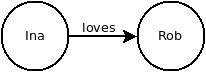
\includegraphics[width=120mm]{./P1.start/01_node-to-node.jpeg}
    \caption{A simple link}
    \label{odb2Nodes}
\end{figure}


\begin{lstlisting}
; 2nodes.cpp

#include <iostream>

#include "generic.h"
#include "odb.h"

auto oOdb = odb::COdb();

int main()
    {
    // 2 people
    oOdb.MakeNode("Ina");
    oOdb.MakeNode("Rob");
    
    // a relation
    oOdb.MakeReason("loves");
    
    // binding
    oOdb.LinkNode2Node("Ina", "loves", "Rob");
    
    // show us
    std::cout << "---------------- all nodes" << '\n';
    for ( auto const & a:oOdb.Nodes() )
        {
        std::cout << *a << '\n';
        }
    }
\end{lstlisting}

Beschreibender Text

\begin{itemize}
\item  create nodes
\item  create reason
\item  link node with reason
\end{itemize}





\end{document}
